\documentclass{article}
\title{Notes for: Proximal Policy Optimization Algorithms\thanks{paper: https://arxiv.org/abs/1707.06347}}
\author{Michael (aka Lisb0n).}
\date{\today}
\usepackage{graphicx}
\usepackage{amsmath}
\usepackage{graphicx}
\usepackage{amsfonts}
\usepackage{xcolor}

\begin{document}
\maketitle

\section{High Level and Motivations}

\subsection{Motivational example}
\begin{enumerate}
    \item You're the proud owner of a RL-robot 9000 (it's a shiny new model and you've heard it's much better than those "control-robot 2000s") The RL-robot 9000 is very expensive (you've saved up the cash to buy this thing over the past 3 years!!)
    \item The robot is tasked with collecting gold coins
    \item The robot is generally quite successful at its task of coin collection, sometimes it finds coins on the street, sometimes if finds coins under the couch.
    \item When the agent finds a gold coin you reward it with a treat to incentivise the robot to collect more coins in the future.
    \item Every now and then the agent will pause and think about all the treats it received recently, it considers what it could do better next time to gain more treats.
    \item You take your robot on a field-trip to the zoo to see the sites and perhaps find some more coins.
    \item It knows that coins are often found around humans so it goes and searches under a few benches and looks at the floor amongst crowds of people. It finds a few coins, you give the robot its treat and it becomes more incentivised to search around people.
    \item You go off to look at the flamingo enclosure and let your robot run free collecting coins.
    \item A small while later your robot comes back with a unusually large sack of gold coins, you give the robot a funny look but provide it with its (large) reward, you carry on to the lizard enclosure and let the robot roam free again.
    \item Some time passes while you are enjoy the sights of the different lizards and lizard-like creatures. You hear a sound from behind and turn to see that a police guard is carrying a now beat up version of your robot, the baton marks on the robot match the baton the guard is carrying. 
    \item The guard explains that the robot was accosting people and demanding they empty their wallets or it would throw them into the lion pit. If you knew this was happening you absolutely would've put a stop to it.
    
\paragraph{A possible cause} The first time the robot returned with the sack of coins you unknowingly rewarded its action of demanding payment from people, importantly, this time, clearly the guards weren't watching. When placed in a similar circumstance, it thought back to last time \emph{my owner rewarded me BIG TIME last time when I accosted people, I'm going to start doing this at a larger scale!!} Unfortuantly for your robot, the guards noticed the trail of crying children and upset families and thus beat your robot to a pulp when it was captured.
\paragraph{An alternate ending} If the guards spotted the robot the first time it accosted someone (it only did it once) they may have been more lenient and simply given the robot a light knock over the head (and thus the robot would quickly learnt to not accost people).
\paragraph{A possible solution} If the agent had some limit to how its behaviour could change to attain more of reward after receiving a positive (or negative [although this isn't in this example]) reward it may have only accosted 2 people which may have made the guards more lenient (as opposed to the hundreds of people accosted in the example)

\textbf{This is a motivating example, not actually what happens. What's described here is what TRPO solves but PPO does too.} PPO also enables another key thing to do with enabling training over multiple epochs of minibatches. 

\end{enumerate}

\subsection{What is PPO?}

\paragraph{Proximal Policy Optimization} is, in essence, a unique objective function which your agent attempts to maximise. This is opposed to simply maximising your expected return as is done in normal policy gradient methods.

Here's a spoiler of what we end up maximising:
\[L_t^{\text{CLIP + VF + S}} (\theta) = \hat{\mathbb{E}} \left [ L_t^{\text{CLIP}}(\theta) - c_1 L_t^{\text{VF}} + c_2 S[\pi_\theta](s_t) \right] \]

\paragraph{The main aims} of PPO were \textbf{not} to build a "better" or "more accurate" optimisation method or function. The primary driver for the development of PPO was to be a \textbf{simple to implement} alternative to TRPO (Trust Region Policy Optimization). \\ 
It's worth noting that PPO also \textbf{beats TRPO} empirically on \emph{most} tasks. 

\paragraph{Batch training?} One of the key benefits of the PPO algorithm (alongside matching TRPO's special "trust region" ideas [discussed later]) is that PPO is highly robust against "overfitting" to policy changes per se.  This means that you can collect a lot of data from one policy and then use that for optimization and be A-OK. 

\section{Body}

\subsection{Old methods}

\subsubsection{Policy Gradient}

This is the most basic method. It works by computing an estimator of the policy gradient (policy parameters w.r.t. expected return) and then attempting to find the maximum of this using a gradient ascent algorithm.

E.g. the standard gradient estimator looks like:
\[ \hat{g} = \textcolor{red}{\hat{\mathbb{E}}} \left [ \nabla_\theta \log \textcolor{blue}{\pi_\theta (a_t | s_t)} \textcolor{violet}{\hat{A}_t} \right ] \]

\begin{itemize}
    \item[\textcolor{blue}{\(\pi_\theta\)}] stochastic policy. Think: neural network outputting an action probability.
    \item[\textcolor{red}{\(\hat{\mathbb{Ep[]}}\)}] \emph{Empirical} average over a finite batch of samples.
    \item[\textcolor{violet}{\(\hat{A}_t\)}] Noisy estimate of the advantage function at time \(t\). Think: neural network outputting an advantage estimate.
\end{itemize}
\paragraph{We construct} an objective function which has a gradient of the policy gradient estimator. E.g. \(\hat{g}\) can be obtained by differentiating:
\[L^{PG} (\theta) = \hat{\mathbb{E}}_t \left [ \log\pi_\theta (a_t | s_t) \hat{A}_t \right] \]

\subsection{TRPO}

TRPO is both really useful and also really icky at the same time. This is primarily due to its difficult implementation details. To summarise TRPO, they propose optimizing the following constrained surrogate objective:

\begin{align*}
    \underset{\theta}{\text{maximise}} \;\; &\hat{\mathbb{E}}_{t} \left [ \frac{{\pi_\theta} (a_t|s_t)}{{\pi_{\theta_{old}}} (a_t|s_t)} \hat{A_t} \right] \\
    \text{subject to} \;\; &\hat{\mathbb{E}}_{t} \left [ KL \left[  \pi_{\theta_{old}} (\cdot|s_t), \pi_{\theta} (\cdot|s_t)\right] \right] \le \delta
\end{align*}

In the TRPO paper they also show you can actually use a penalty term instead of a constraint:
\[
    \underset{\theta}{\text{maximise}} \;\; \hat{\mathbb{E}}_{t} \left [ \frac{{\pi_\theta} (a_t|s_t)}{{\pi_{\theta_{old}}} (a_t|s_t)} \hat{A_t} \right] - \beta \hat{\mathbb{E}}_{t} \left [ KL \left[  \pi_{\theta_{old}} (\cdot|s_t), \pi_{\theta} (\cdot|s_t)\right] \right]
\]

It so happens that it's \emph{really} hard to pick a \(\beta\) that works well on different problems. This is why a hard constraint tends to be used. 

\subsection{Clipped Surrogate Objective: The Main Meal}
\paragraph{If nothing else,} this is the part which is worth understanding. The ``clipped surrogate objective" is pretty much the entire PPO idea.
\paragraph{This is also} the best place to ask questions (if you think you have any).

\paragraph{How to come up with the idea of PPO yourself.} To help bring an intuition and rationale for the PPO algorithm I'll try to describe what you're looking for.

\paragraph{Let's say} we've collected some samples from the environment under policy \( \pi_{\theta_{\text{old}}} \) and we now want to update/create a \( \pi_\theta\) according to these samples.

\paragraph{At each update step we must consider 3 things:}
\begin{enumerate}
    \item \textcolor{blue}{ What was the probability of selecting this action AT THE TIME OF SELECTION (under the \textbf{old policy \( \pi_{\theta_{\text{old}}} \)} ) }
    \item \textcolor{blue}{What is the probability of selecting this action UNDER THE \textbf{new policy \( \pi_\theta\) } }
    \item \textcolor{violet}{The \textbf{advantage estimate \( \hat{A}_t \)} of that action taken (this is computed right after taking this action by, typically, a neural network)}
\end{enumerate}

\textcolor{blue}{\subsubsection{Why do we need the probabilities of taking the action under the old and new policies?}}
Because we want to compute some sort of measure of how different the decision of the new policy is to the old policy. We can do this by letting:
\[r_t(\theta) = \frac{\pi_\theta (a_t | s_t)}{\pi_{\theta_{\text{old}}} (a_t | s_t)}\]
\[\Rightarrow r(\theta_\text{old}) = 1\]

\paragraph{Let's linger on this} If the new policy will select the action with a much greater probability than the old policy, i.e. \(\pi_\theta (a_t | s_t) > \pi_{\theta_{\text{old}}} (a_t | s_t)\) then \(r(\theta)\) will be \textbf{greater than 1}. \\ The opposite is also true: \(\pi_\theta (a_t | s_t) < \pi_{\theta_{\text{old}}} (a_t | s_t)\) then \(r(\theta)\) will be \textbf{less than 1}.

It's worth noting that this is not the same as the computing the difference between policy distributions or something like that (therefore no KL divergences are necessary)\textbf{*}. We are simply measuring the probability ratio of one action under one policy over another policy.

\paragraph{*}This CAN be replaced by a KL divergence term, but then we're stepping awfully close to TRPO. They also performed empirical tests and showed that the KL divergence stuff worsens performance (thank god - we don't need to deal with that).

\textcolor{violet}{\subsubsection{Why do we need the advantage estimate of the action taken?}}

At each time step we need access to what the estimated advantage was. For example, while running the policy we may follow the following sequence:
\begin{enumerate}
    \item Observe the environment
    \item \emph{Estimate advantage of previous action \(\hat{A}_{n-1}\) and store it somewhere safe} 
    \item Select action based on observation according to the policy
    \item Take the action selected 
    \item Make new observation
    \item \emph{Estimate the advantage of the action \(\hat{A}_{n}\) we just took and store it somewhere safe.} 
\end{enumerate}

Note: we use a neural network to estimate \(\hat{A}_{t}\), because neural networks are imperfect/noisy our Advantage estimates will be imperfect/noisy too. 

We need these estimates because \textbf{this is what we will use to update the policy}. The advantage estimator is what is updated based on empirical evidence, i.e. this is what is actually updated based on rewards observed.

When \(\hat{A}_{t}\) is positive, the action selected was better than expected.
When \(\hat{A}_{t}\) is negative, the action selected was worse than expected.

\subsubsection{Putting the pieces together}

There are 4 interesting circumstances when updating our model:


\begin{center}
    \begin{tabular}{ c|c|c| } 
    & \(\hat{A}_{t} > 0\)  & \(\hat{A}_{t} < 0\)  \\
    \hline
    \(r_t (\theta) > 1 \) & CASE 1  & CASE 2 \\
    \hline
    \(r_t (\theta) < 1 \) & CASE 3  & CASE 4
\end{tabular}
\end{center}

In TRPO, \(\hat{\mathbb{E}} \left [ r_t(\theta) \hat{A}_t \right]\) this is the objective we optimize for (ignoring the constraint). Therefore we'll use this as the method 

\begin{itemize}
    \item[CASE 1] Under the new policy we take this action more frequently and the advantage is positive! This suggests the policy should take this action EVEN MORE!
    \item[CASE 2] Under the new policy we take this action more frequently but the advantage is negative so we should take this action less.
    \item[CASE 3] Under the new policy we take this action less frequently but the advantage is positive so we should take the action more.
    \item[CASE 4] Under the new policy we take the action less frequently and the advantage function is negative! This suggests the policy should take this action EVEN LESS!
\end{itemize}

\paragraph{An insight} 2 of these cases make the new policy closer to the old policy while 2 drive the new policy further away. Can you identify which?\footnote{CASE 2 and 3 make the new policy closer to the old policy} While we do want the new policy to be different from the old policy (otherwise what's the point of training), we don't want it to get too far away (we might be ``overfitting" the new policy on the noisy advantage estimates).

\paragraph{What we need} is something which allows the new policy to drift closer to the old policy (we don't care about the potential performance loss) while limiting how far it can drift away from the old policy.

\[
    L^{\text{CLIP}} (\theta) = \hat{\mathbb{E}}_t \left [ \min(  r_t (\theta) \hat{A}_t , \text{clip}(r_t (\theta), 1 - \epsilon, 1 + \epsilon)\hat{A}_t ) \right]
\]
where \(\epsilon\) is a hyperparameter which is usually set to \(\approx 0.2\) It represents how ``far'' the new policy is allowed to drift away from the old policy.

\paragraph{Math translation:}
\paragraph{}remember:
\[r_t(\theta) = \frac{\pi_\theta (a_t | s_t)}{\pi_{\theta_{\text{old}}} (a_t | s_t)}\]

\paragraph{LET} \(\epsilon = 0.2\). Each cell value is the clipped objective:
\begin{center}
    \begin{tabular}{ c|c|c| } 
    & \(\hat{A}_{t} > 0\)  & \(\hat{A}_{t} < 0\)  \\
    \hline
    \(r_t (\theta) \) is large & \(1.2 \times \hat{A}_t\)  & \(r_t(\theta) \times \hat{A}_t\)  \\
    \hline
    \(r_t (\theta) \) is small & \(r_t(\theta) \times \hat{A}_t\) & \(0.8 \times \hat{A}_t\) 
\end{tabular}
\end{center}
    
Hopefully you can see that this outcome satisfies what we wanted. 

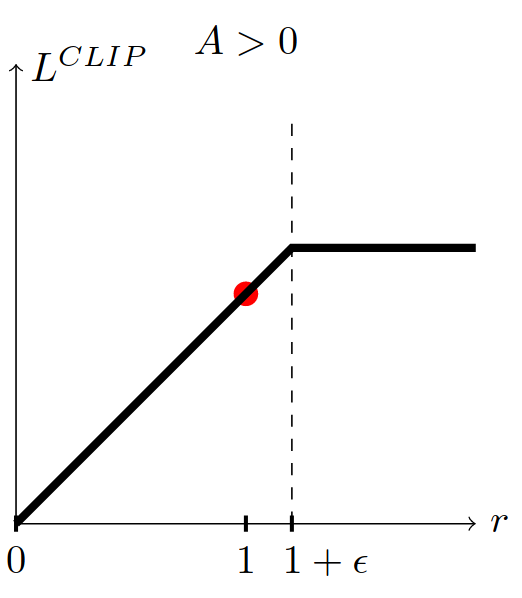
\includegraphics[scale=0.4]{fig1.png}
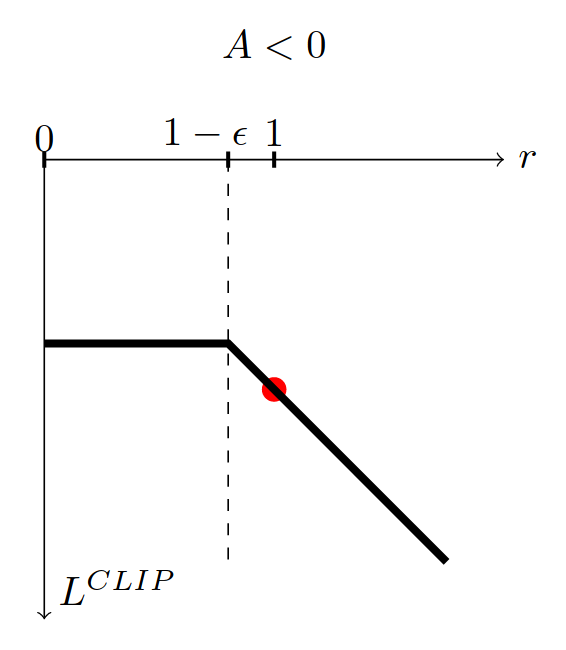
\includegraphics[scale=0.4]{fig2.png}

\section{Other bits}

time ran out, please ask about other stuff. I will try to discuss what I think I missed from this:

\[L_t^{\text{CLIP + VF + S}} (\theta) = \hat{\mathbb{E}} \left [ L_t^{\text{CLIP}}(\theta) - c_1 L_t^{\text{VF}} + c_2 S[\pi_\theta](s_t) \right] \]

\end{document}